\chapter{Diseño y Desarrollo}
\label{ch:modelo}

Este capítulo describirá el diseño y desarrollo del modelo de predicción de demanda y optimización de ingresos. El primer paso será presentar los \emph{data sets} utilizados. El segundo paso consistirá en describir el modelo, sus módulos, el funcionamiento y la arquitectura.

\section*{Data Sets}

\subsection*{Detalle de reservaciones}

Para la construcción del modelo de predicción de demanda se utilizaron tres data sets que contienen la información suficiente para poder hacer un pronóstico efectivo de la demanda de una propiedad.

El primer data set utilizado fue extraído directamente del sistema de gestión de propiedades y contiene información de todas las reservaciones marcadas en los libros de la propiedad, así como la información de las estancias pasadas. A continuación se presenta a detalle la información contenida en este data set, el diccionario de datos y un breve resumen de la información en cada una de las columnas.

\subsubsection*{Diccionario de Datos}

A continuación se presenta el diccionario de datos del \emph{data set} que contiene la información detallada de las reservaciones:

\begin{itemize}
  \item rsrv\_code: Código de confirmación de la reservación
  \item date\_create: Fecha y hora de creación de la reserva
  \item date\_in: Fecha de llegada a la propiedad
  \item date\_out: Fecha de salida de la propiedad
  \item nights: Número de noches de la reservación en el hotel
  \item prop\_code: Código de la propiedad dentro del sistema de gestión de propiedades
  \item mkt\_sgm: Segmento de mercado del huésped amparado en la reservación
  \item Dia\_Sem: Día de la semana de la fecha de llegada del huésped
  \item rate\_code: Código de tarifa
  \item bucket: Categoría de tarifa
  \item Ingresos: Ingresos obtenidos por la renta habitación de la reservación
  \item rsrv\_src: Canal de generación de la reservación
  \item rsrv\_type: Tipo de reservación
  \item room\_type: Tipo de habitación
  \item PAX: Número de personas amparadas por la reservación
\end{itemize}

\subsubsection*{Resumen de datos}

\begin{verbatim}
##    rsrv_code        date_create                 
##  Min.   :6265739   Min.   :2016-07-20 18:31:59  
##  1st Qu.:7499788   1st Qu.:2017-03-27 10:10:09  
##  Median :7999769   Median :2017-06-30 12:12:57  
##  Mean   :8007253   Mean   :2017-06-27 13:38:02  
##  3rd Qu.:8505582   3rd Qu.:2017-09-27 13:22:36  
##  Max.   :9053354   Max.   :2018-01-01 03:08:21  
##     date_in                   
##  Min.   :2017-01-01 00:00:00  
##  1st Qu.:2017-04-04 00:00:00  
##  Median :2017-07-06 00:00:00  
##  Mean   :2017-07-06 02:18:17  
##  3rd Qu.:2017-10-08 00:00:00  
##  Max.   :2017-12-31 00:00:00  
##     date_out                       nights 
##  Min.   :2017-01-02 00:00:00   Min.   :1  
##  1st Qu.:2017-04-05 00:00:00   1st Qu.:1  
##  Median :2017-07-07 00:00:00   Median :1  
##  Mean   :2017-07-07 02:18:17   Mean   :1  
##  3rd Qu.:2017-10-09 00:00:00   3rd Qu.:1  
##  Max.   :2018-01-01 00:00:00   Max.   :1  
##   prop_code           mkt_sgm            Dia_Sem         
##  Length:44391       Length:44391       Length:44391      
##  Class :character   Class :character   Class :character  
##  Mode  :character   Mode  :character   Mode  :character  
##                                                          
##                                                          
##                                                          
##   rate_code            bucket             Ingresos   
##  Length:44391       Length:44391       Min.   :   0  
##  Class :character   Class :character   1st Qu.:1200  
##  Mode  :character   Mode  :character   Median :1462  
##                                        Mean   :1449  
##                                        3rd Qu.:1658  
##                                        Max.   :3900  
##    rsrv_src          rsrv_type          room_type        
##  Length:44391       Length:44391       Length:44391      
##  Class :character   Class :character   Class :character  
##  Mode  :character   Mode  :character   Mode  :character  
##                                                          
##                                                          
##                                                          
##       pax       
##  Min.   :0.000  
##  1st Qu.:1.000  
##  Median :1.000  
##  Mean   :1.271  
##  3rd Qu.:1.000  
##  Max.   :5.000
\end{verbatim}

Es importante resaltar que los datos fueron trabajados para presentarse de manera desagregada, es decir, si una reservación ampara una estancia de 5 noches, en el \emph{data set final} se presenta un registro por cada noche de la estancia, por ejemplo:

\begin{knitrout}
\definecolor{shadecolor}{rgb}{0.969, 0.969, 0.969}\color{fgcolor}\begin{table}[H]
\centering\rowcolors{2}{gray!6}{white}

\begin{tabular}{r|l|l|l|r|l}
\hiderowcolors
\hline
rsrv\_code & date\_create & date\_in & date\_out & nights & room\_type\\
\hline
\showrowcolors
6265739 & 2016-07-20 18:31:59 & 2017-04-07 & 2017-04-08 & 1 & NSK\\
\hline
6265739 & 2016-07-20 18:31:59 & 2017-04-08 & 2017-04-09 & 1 & NSK\\
\hline
6265739 & 2016-07-20 18:31:59 & 2017-04-09 & 2017-04-10 & 1 & NSK\\
\hline
6265739 & 2016-07-20 18:31:59 & 2017-04-10 & 2017-04-11 & 1 & NSK\\
\hline
6265739 & 2016-07-20 18:31:59 & 2017-04-11 & 2017-04-12 & 1 & NSK\\
\hline
6265739 & 2016-07-20 18:31:59 & 2017-04-12 & 2017-04-13 & 1 & NSK\\
\hline
\end{tabular}
\rowcolors{2}{white}{white}
\end{table}
\end{knitrout}

Como se puede observar, el número de reservación es el mismo en los seis registros, lo mismo ocurre con la fecha de creación, las noches y el tipo de habitación, sin embargo, la fecha de entrada y la fecha de salida va cambiando en cada registro.

\subsubsection*{Curvas de Pickup}

Del data set anterior podemos obtener las curvas de pickup del hotel. Estas curvas describen el comportamiento de las reservaciones para la propiedad en cuestión ya que mediante ellas podemos saber con cuanto tiempo de anticipación los huéspedes comienzan a reservar una habitación en la propiedad. A continuación se muestran las curvas de pickup para esta propiedad:

\definecolor{shadecolor}{rgb}{0.969, 0.969, 0.969}\color{fgcolor}
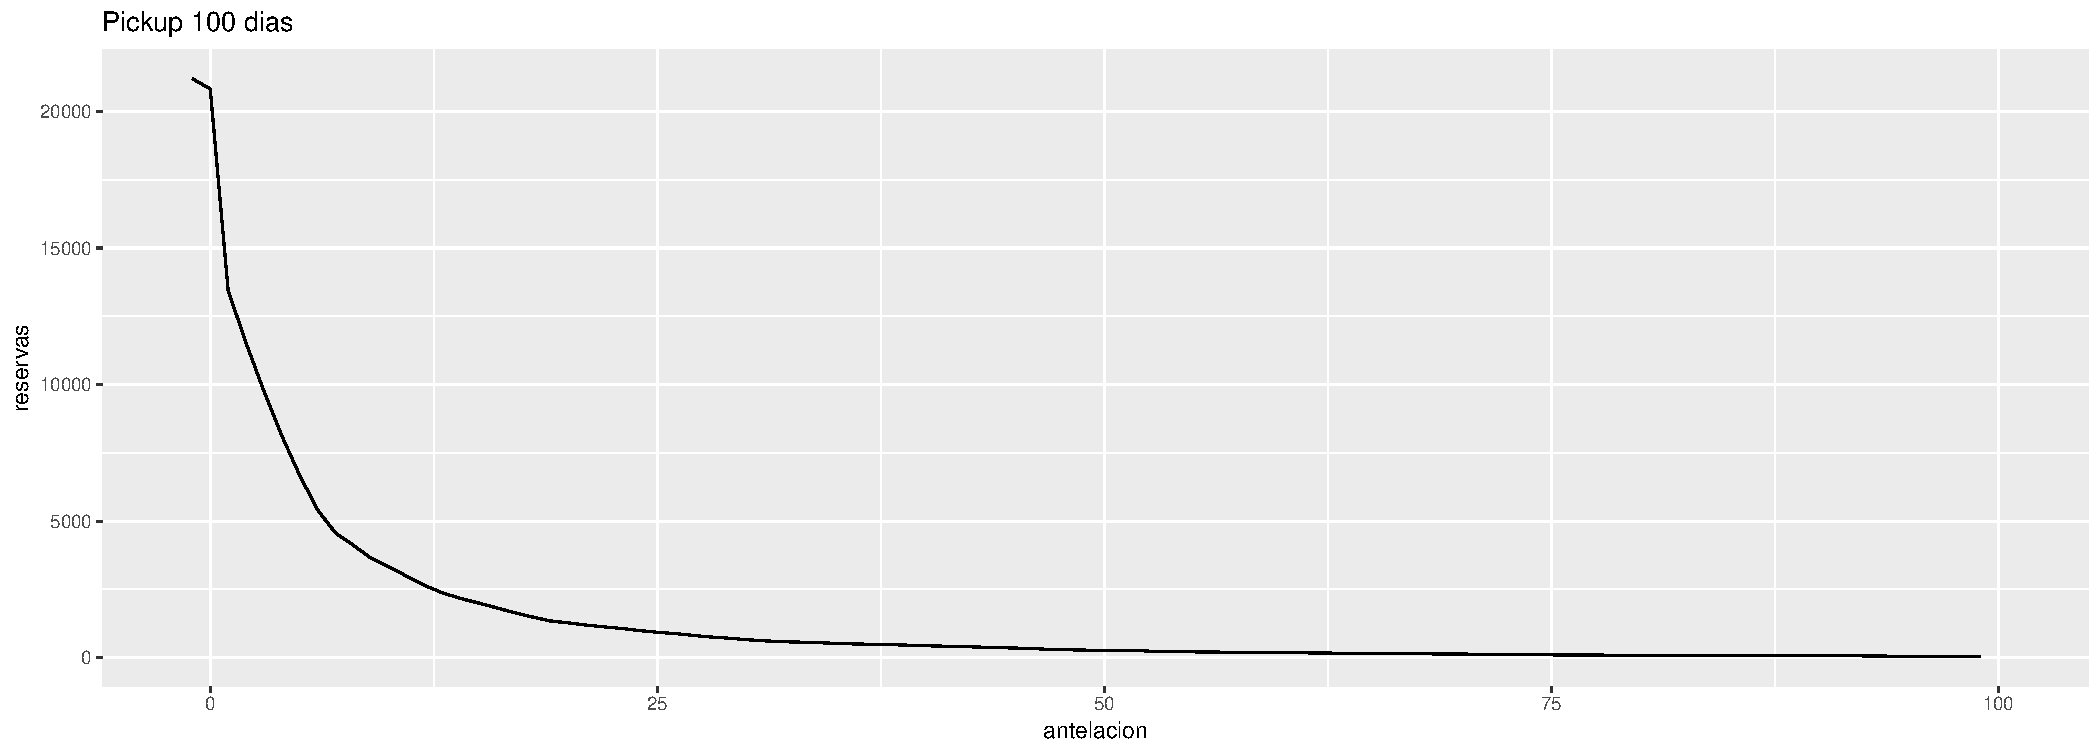
\includegraphics[width=\maxwidth]{Figures/pickup-1} 

\definecolor{shadecolor}{rgb}{0.969, 0.969, 0.969}\color{fgcolor}
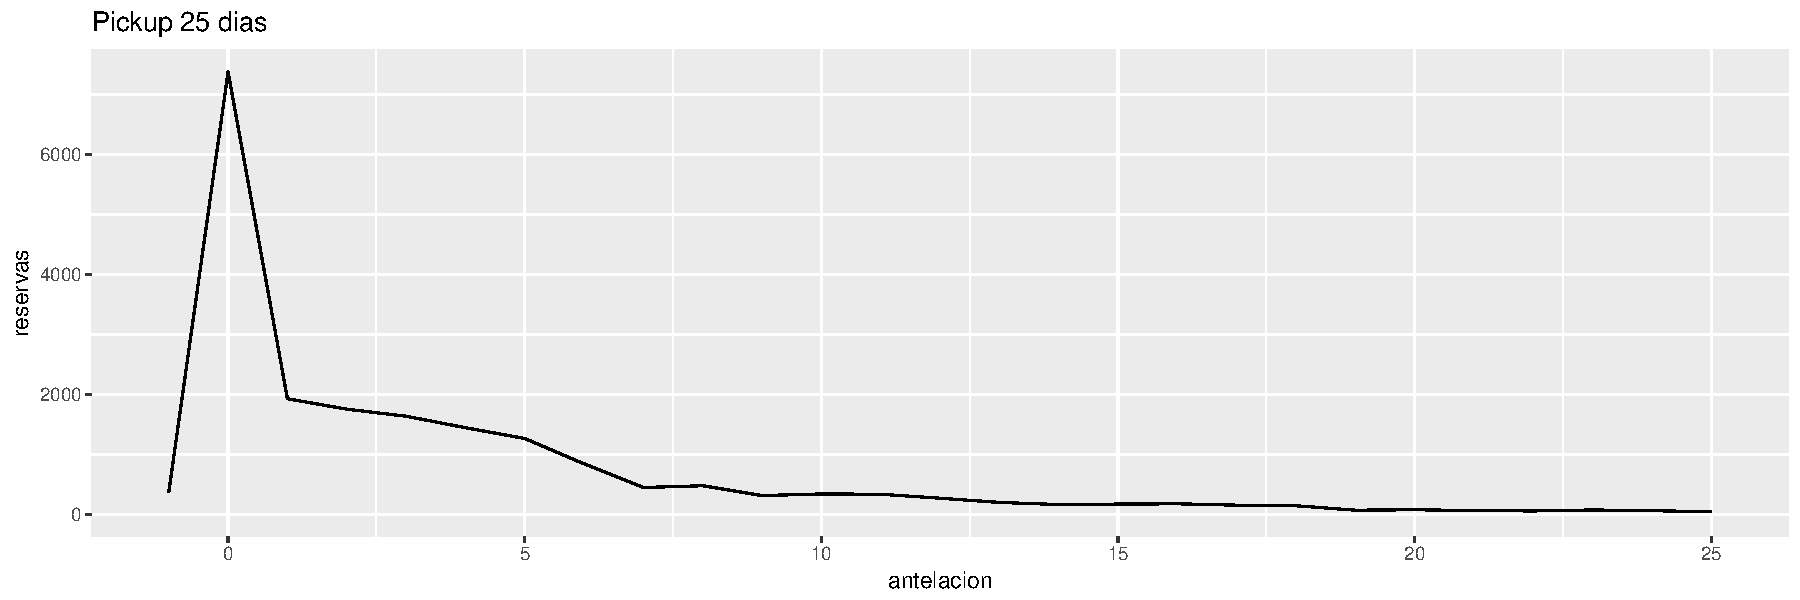
\includegraphics[width=\maxwidth]{figures/pickupzoom-1} 

Analizando las gráficas presentadas anteriormente podemos concluír que la demanda de esta propiedad comienza 25 días antes de la llegada del huésped al hotel, e incrementa considerablemente 5 días antes de la llegada del huésped al hotel. Este dato nos indica que el huésped comienza a buscar una habitación dentro de esta propiedad en un lapso no mayor a 25 días antes de emprender su viaje.

Las curvas de \emph{pickup} son importantes dentro del proceso de toma de decisiones ya que le indican al equipo que gestiona la propiedad el tiempo de antelación con el cual deberían llevar a cabo las acciones necesarias para poder optimizar el ingreso generado por la renta de habitaciones.

\subsection*{Ocupación de la propiedad}

El segundo \emph{data set} con el que se trabajó contiene las líneas de tiempo de los níveles de ocupación de la propiedad. Este set de datos es de suma importancia ya que proporciona información relevante con respecto a las temporalidades del hotel, mismas que deben ser reflejadas en el resultado del modelo.

Las temporalidades del hotel pueden ser desde periodos con alta o baja ocupación, inclusive por día de la semana ya que al ser un hotel enfocado a viajes de negocio, se esperaría tener una alta ocupación los días laborales (Lunes a Jueves) y una baja ocupación los fines de semana (Viernes a Domingo).

A continuación se presentan un par de gráficas que describen el contenido del \emph{data set} en cuestión:

\definecolor{shadecolor}{rgb}{0.969, 0.969, 0.969}\color{fgcolor}
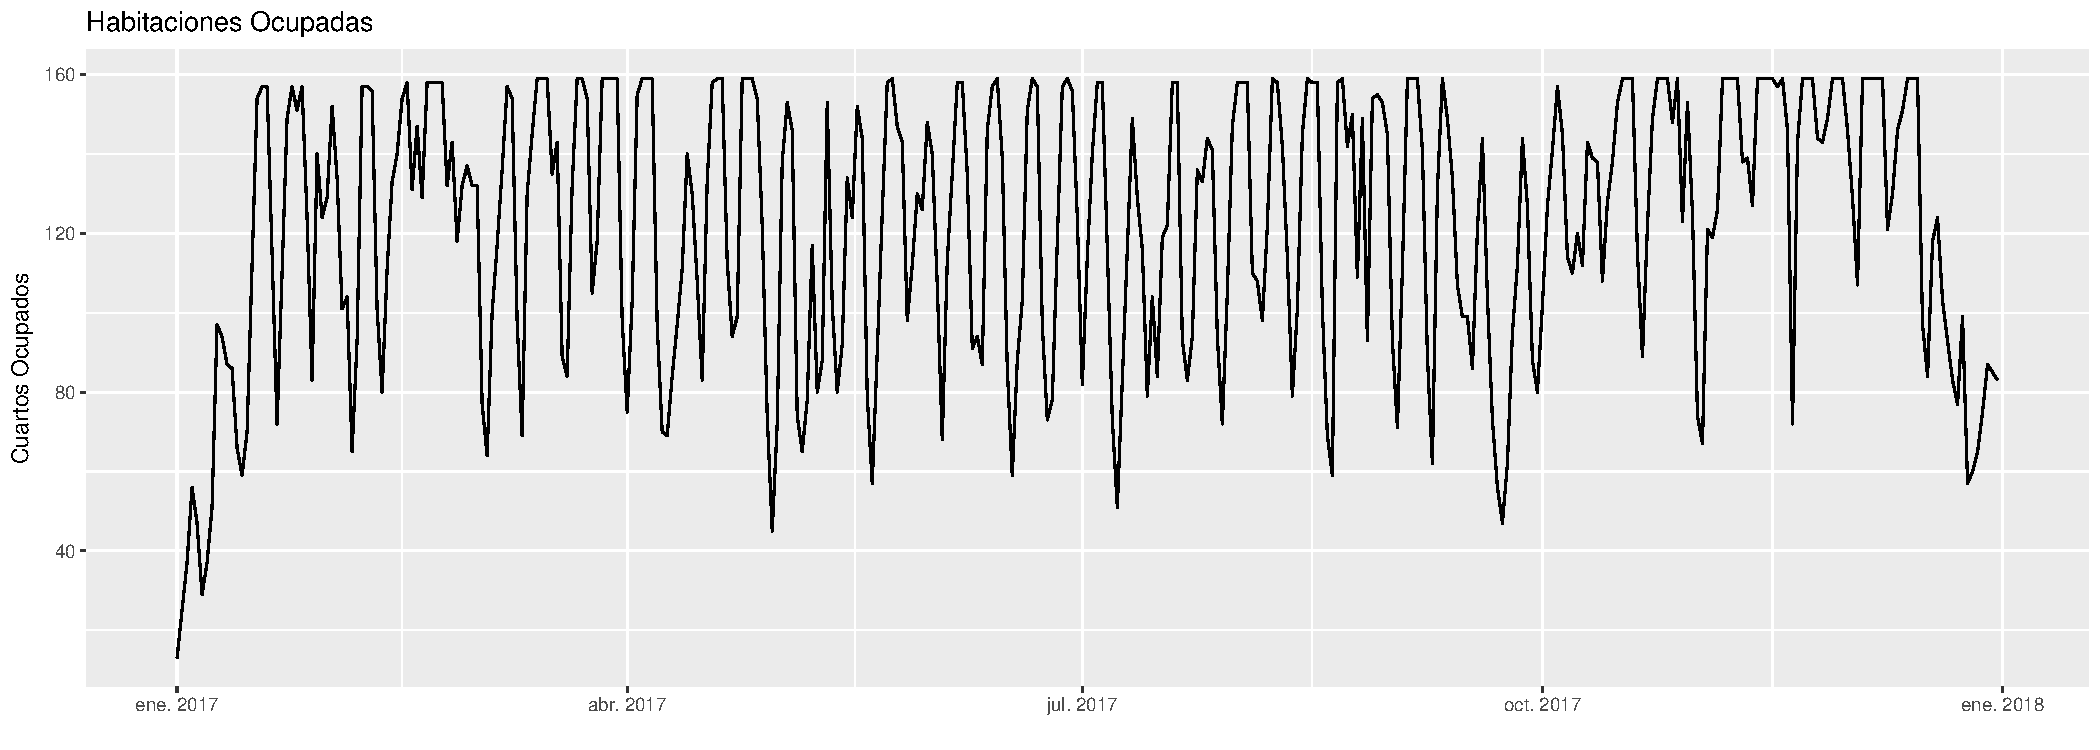
\includegraphics[width=\maxwidth]{figures/HabitacionesOcupadas-1} 

\definecolor{shadecolor}{rgb}{0.969, 0.969, 0.969}\color{fgcolor}
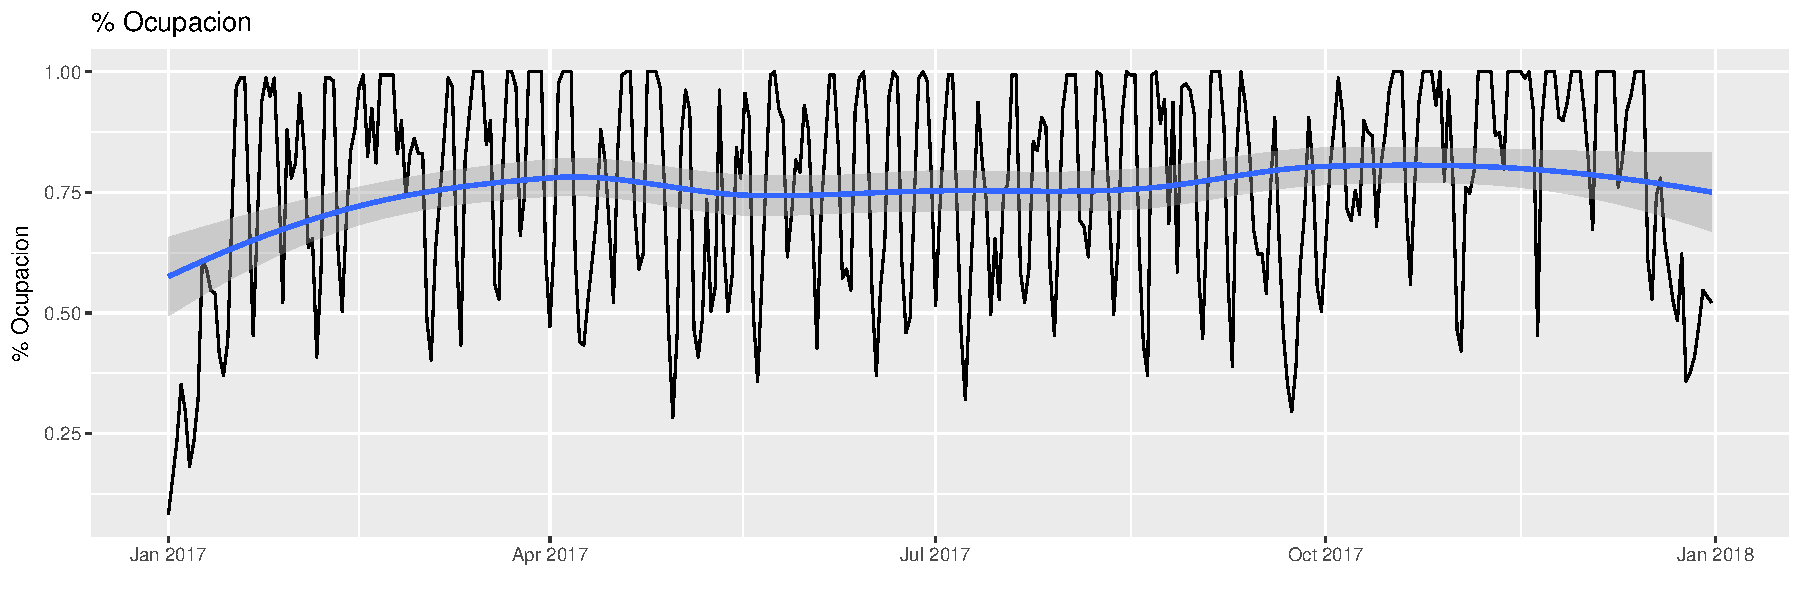
\includegraphics[width=\maxwidth]{Figures/Ocupacion-1} 

Como se puede observar en las gráficas presentadas anteriormente, esta propiedad tiene niveles de ocupación alrededor del 75\% llegando en repetidas ocasiones al 100\% de ocupación. Las caídas en los níveles de ocupación ocurren los fines de semana, lo cual confirma que el mercado objetivo de la propiedad estudiada es el turismo de negocios.

A continuación se presenta una gráfica de níveles de ocupación por día de la semana:

\definecolor{shadecolor}{rgb}{0.969, 0.969, 0.969}\color{fgcolor}
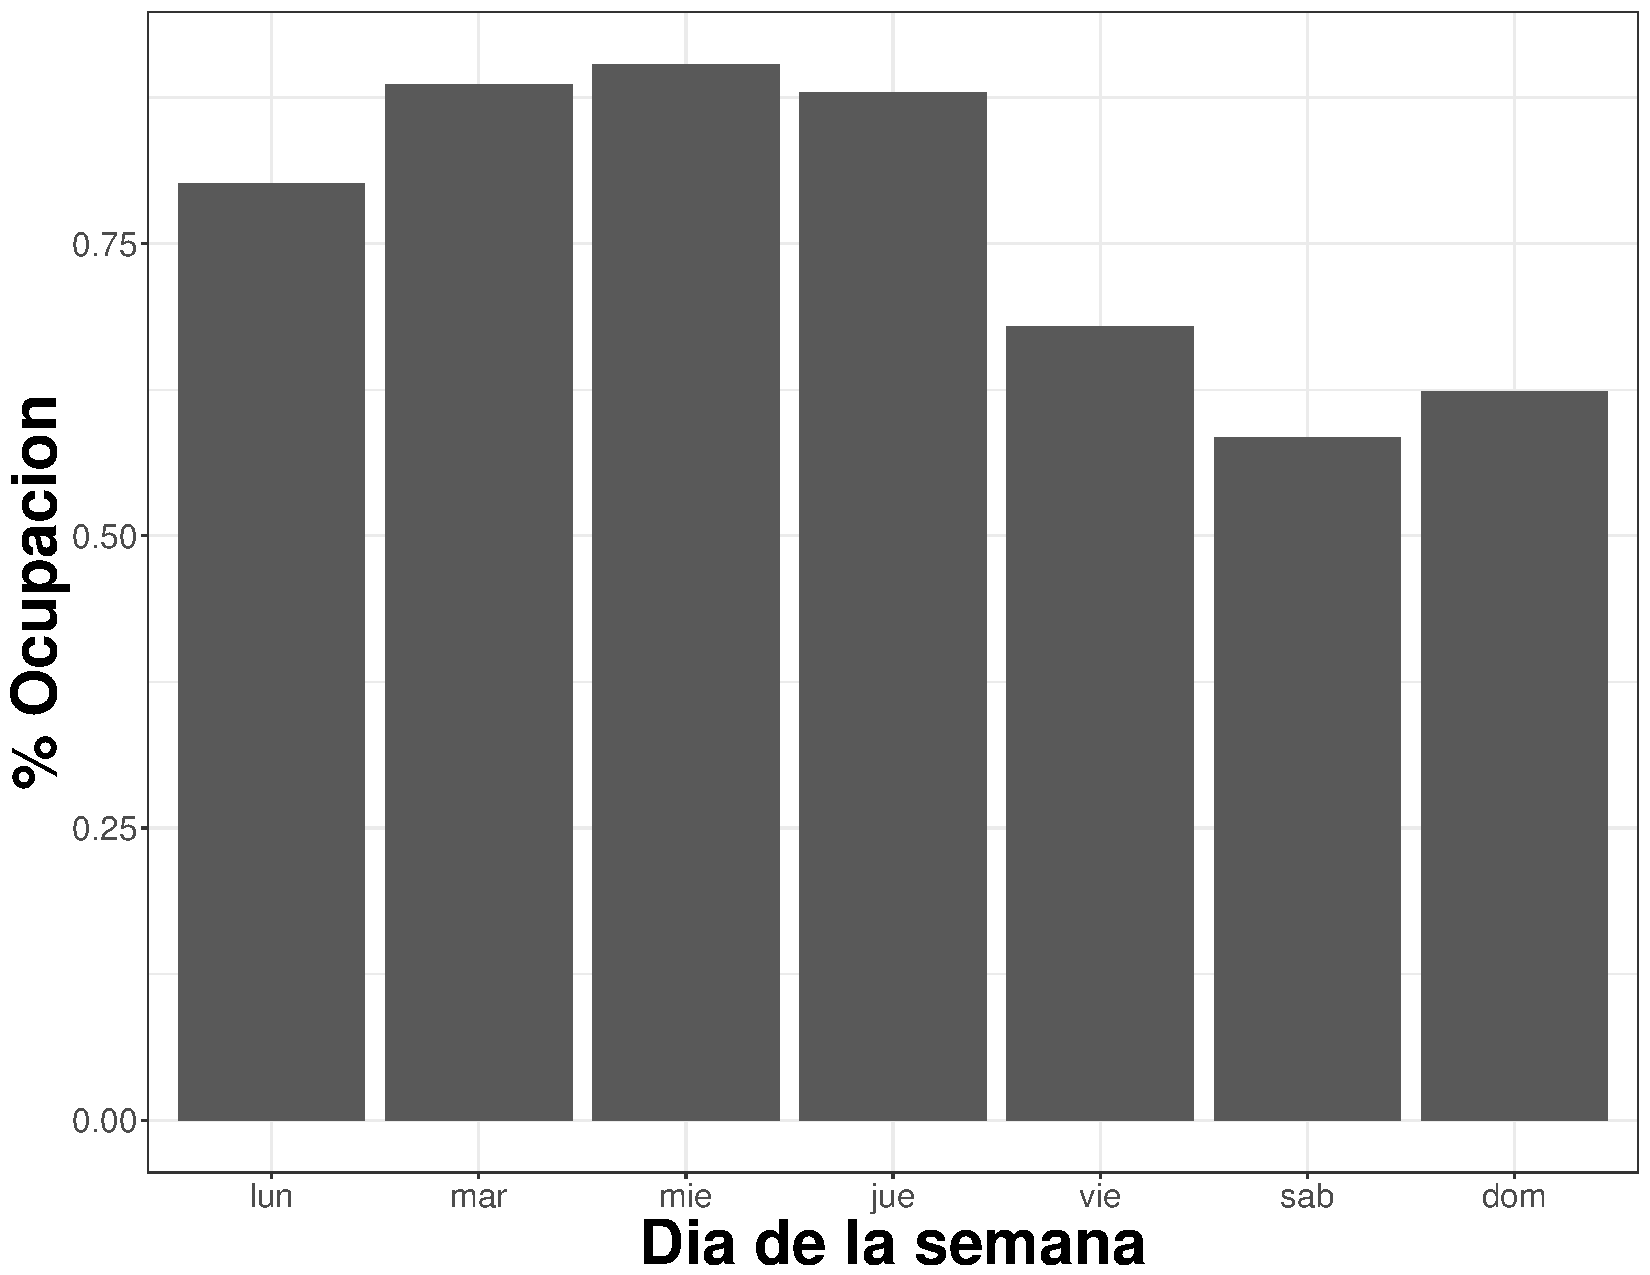
\includegraphics[width=\maxwidth]{Figures/Ocupacion_Dia_Semana-1} 



